\chapter{「じぷり」について}

\section{「じぷり」の概要}%例:レビュー内容
%必要ならここに大見出しの内容
%必要なら下のsubsectionを用いて小見出しをつかう
%\subsection{ここに小見出し}%:発表技法について
本プロジェクトで開発しているHTML5ハイブリッドアプリケーション「じぷり」は, 陣川あさひ町会が企画, 運営するイベント情報の発信, 発信されたイベントへの参加申し込み, 雨天延期などの陣川あさひ町会役員による緊急連絡が可能となるアプリケーションである. このアプリケーションの名称は, 「陣川」という地域の名称と, 「アプリケーション」を組み合わせたものである. 本アプリケーションの目標は, 陣川あさひ町会のイベント開催に関する問題を解決することである. 主な使用場面は新規イベントの開催が決定してから, 当日のイベント終了までを想定している. 既存の他のアプリケーションと比較した際の優位性として, 2点挙げられる. 1つ目は, イベント情報を発信する際に, 過去のイベント情報から生成されたテンプレートを用いることで, 次回以降の入力の手間を省くことができる点である. 2つ目は, 陣川あさひ町会役員にヒアリングを重ねた結果, 町会が本当に必要とする機能を実装している点である. 「じぷり」では対象とするユーザを, 町民, 役員, 管理者に属性分けをした. 管理者とは, 役員の中でもスマートフォンの操作に慣れている人のことである. このようにした理由は, 町会にヒアリングをした際に, 役員の中には上手くアプリケーションを操作できないと考えられるユーザがいるため, 誤った情報を発信するといったリスクを挙げられたからである. そのため町会と相談した上で、管理者を誰にするかを決めた. 「じぷり」では, アプリケーションの起動時に, ユーザが町民, 役員, 管理者のいずれかであるかを選択する. その結果から本アプリケーションは, 町民が利用する「一般モード」か, 役員が利用する「役員モード」か, 管理者が利用する「管理者モード」に画面の遷移を行う. 「一般モード」では, イベント情報とお知らせの閲覧と, イベントへの参加申し込みを行うことができる. 「役員モード」では, 「一般モード」に加えて役員会議など役員以外にとって必要のない情報も閲覧できる. 「管理者モード」では, イベントの管理機能,お知らせの管理機能, 参加者管理機能も行うことができる. 次節より「じぷり」の各機能について詳しく記述していく.

\section{イベント管理機能}%例:レビュー内容
\subsection{イベント管理機能の概要}%:発表技法について
イベント管理機能とは「管理者モード」の場合のみ利用可能な機能であり, イベント情報の発信と発信した情報の編集, 削除を可能としている. イベント管理機能を実装した理由は, イベントの情報をFacebookやLINE@など複数のサービスを使用して発信していた従来の方式から, 本アプリケーション1つですべてを賄うことを可能とするためである.

\subsection{イベント情報の発信機能}%:発表技法について
イベント一覧リスト画面(図\ref{tab:trans_event}(a))から新規作成ボタンを押すと, 発信するイベント情報の入力画面(図\ref{tab:trans_event}(b))に遷移する. この発信画面では, 入力する情報の属性としてイベント告知用の画像, 担当部名, イベント名, 日程, 場所, 開始時間, 終了時間, 定員, 詳細, 申込締切日, 役員のみに公開の11つに分けた. 役員のみに公開とは, 役員会議など町民にとっては知る必要のないイベント情報を判別するために設けた. これら11つの属性は, ヒアリングを通して定まったものである. 情報を入力した後画面下の作成ボタンを押すことでイベント情報を発信することが可能となる. また, ボタンが押された際に本アプリケーションがインストールされているすべての端末に, イベント情報が発信されたことを伝える通知が行く形式にした. 通知機能については, \ref{func:notice}節で詳しく記述する.

\begin{figure}[htbp]
  \begin{center}
    \begin{tabular}{c}

      % 1
      \begin{minipage}{0.33\hsize}
        \begin{center}
        {\setlength{\fboxsep}{0cm}\fbox{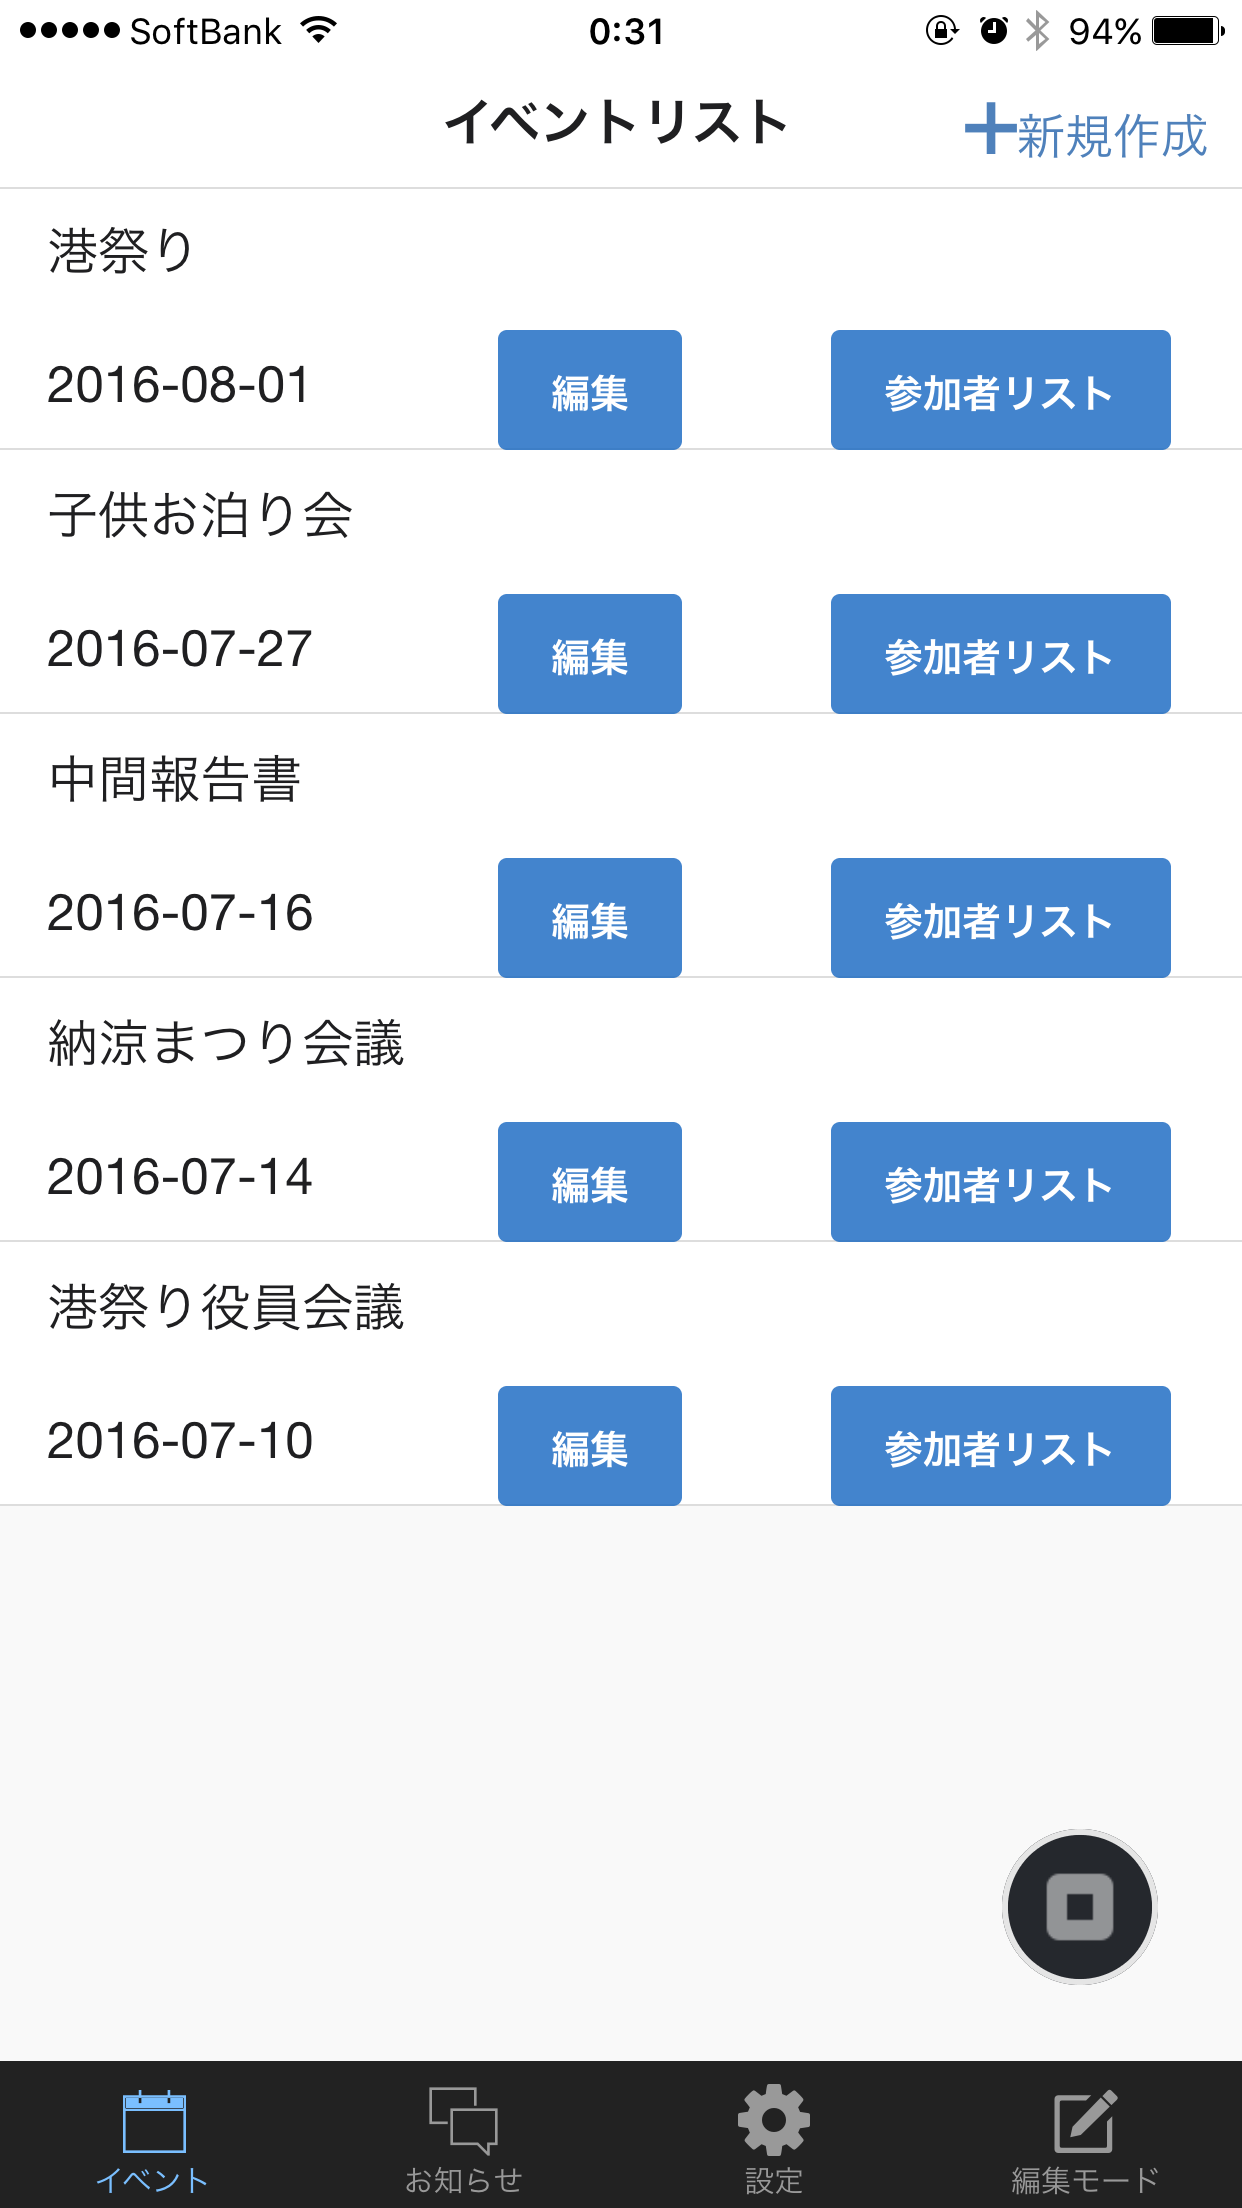
\includegraphics[width=4cm]{event_list.PNG}}}
          \hspace{1cm} %(a)観光スポットの紹介
          {\footnotesize (a)イベント一覧リスト画面}
        \end{center}
      \end{minipage}

      % 2
      \begin{minipage}{0.33\hsize}
        \begin{center}
        {\setlength{\fboxsep}{0cm}\fbox{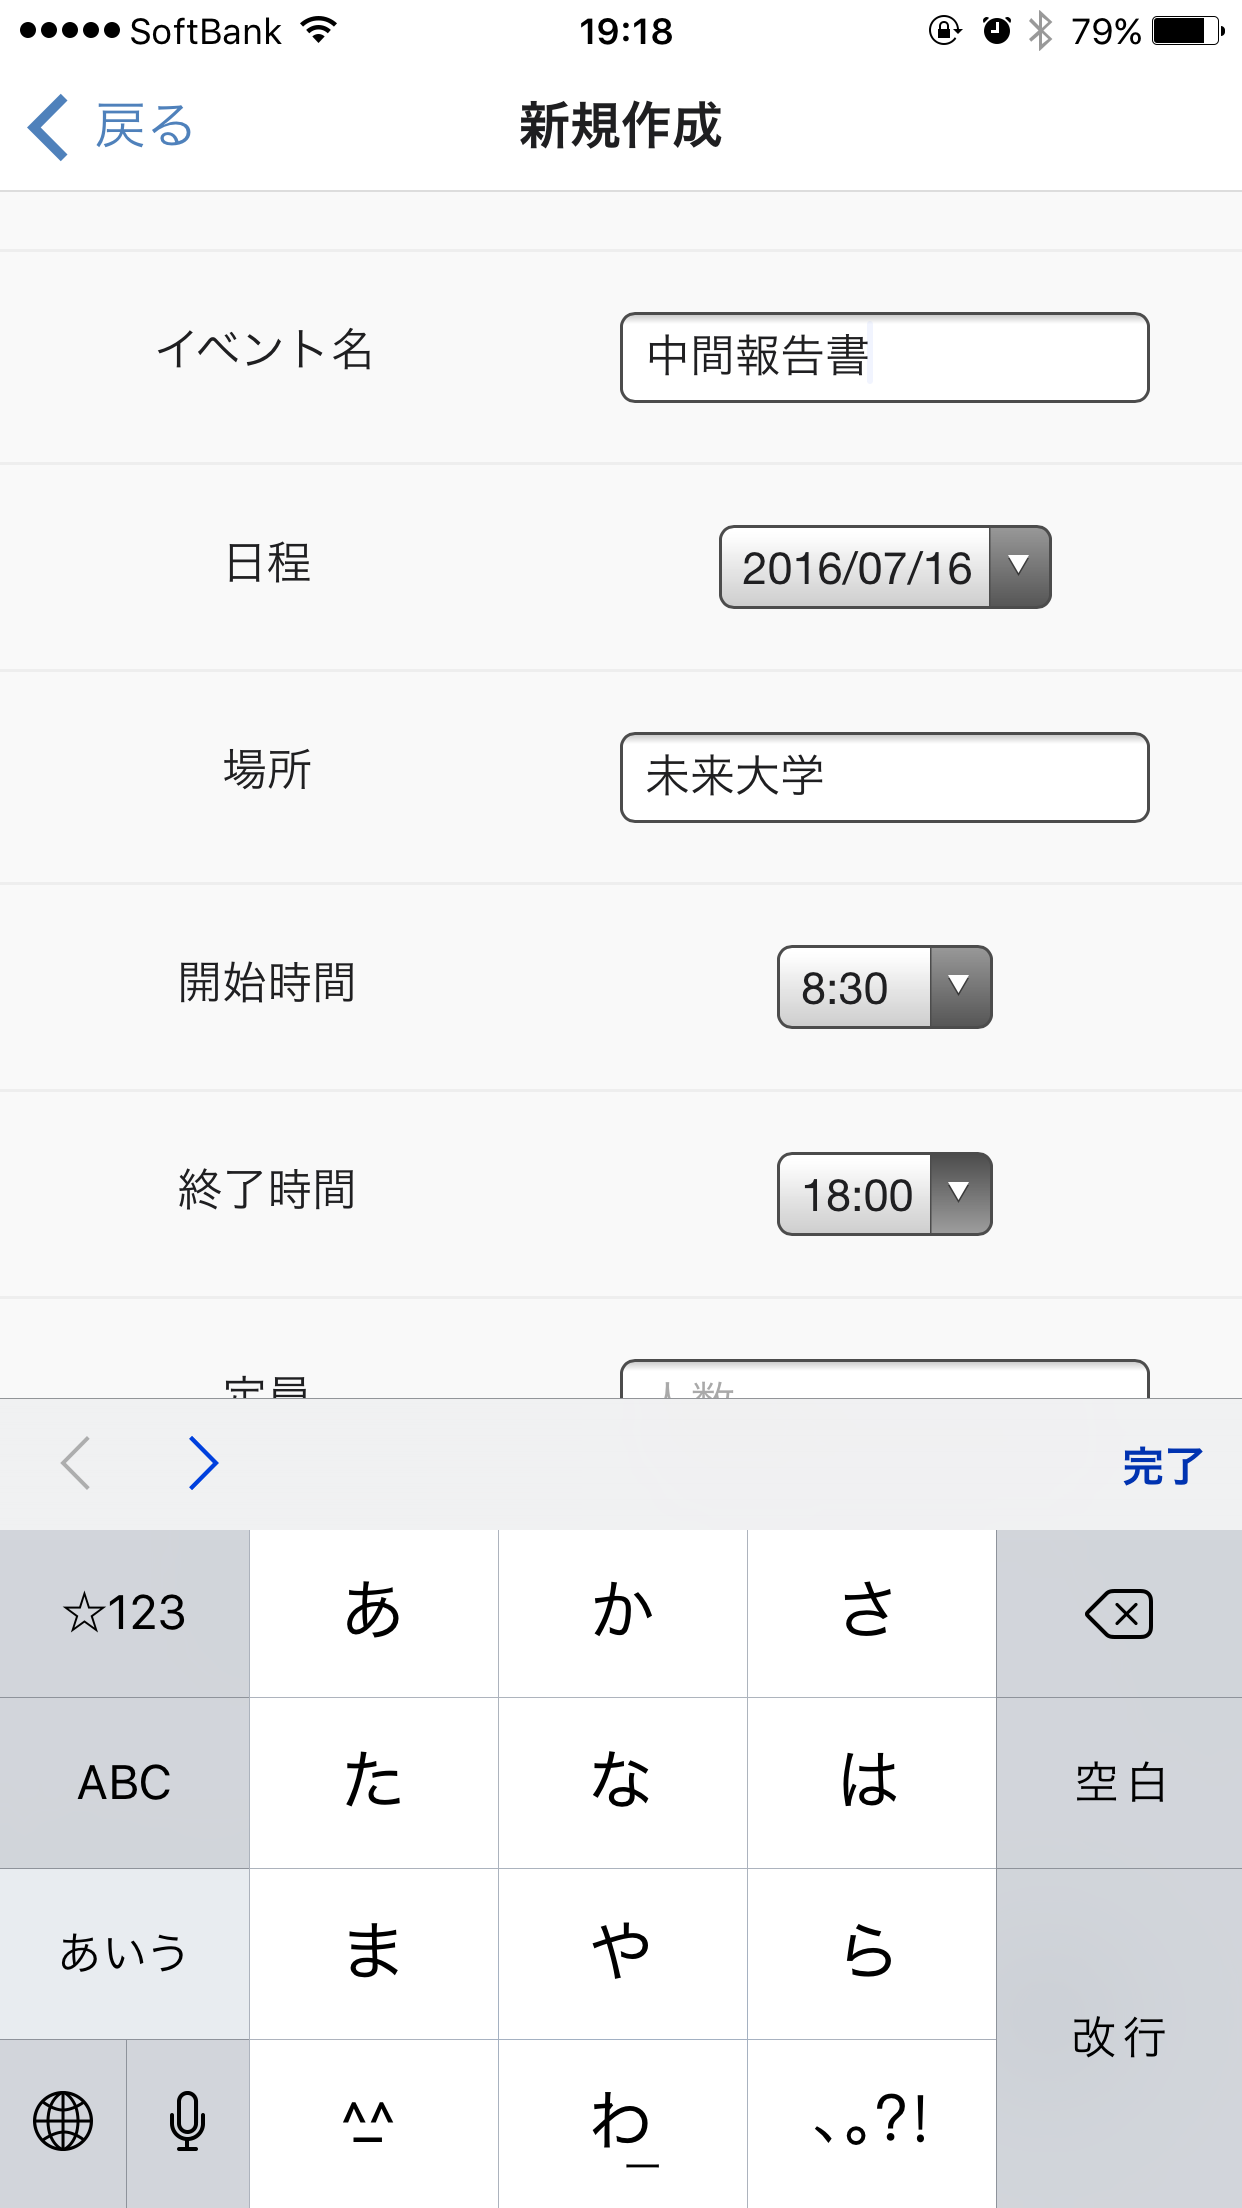
\includegraphics[width=4cm]{event_add.png}}}
          \hspace{1cm}% (b)観光スポットの詳細情報
          {\footnotesize (b)イベント情報の発信画面}
        \end{center}
      \end{minipage}

    \end{tabular}
    \caption{イベント情報の発信}
    \label{tab:trans_event}
  \end{center}
\end{figure}

\subsection{イベント情報の編集機能}%:発表技法について
イベント一覧リスト画面(図\ref{tab:edit_event}(a))から任意のイベントを選択すると, イベント情報の詳細画面(図\ref{tab:edit_event}(b))に遷移する. その後, 右上のメニューボタンからイベントの編集を選択することで, イベント編集画面(図\ref{tab:edit_event}(b))に選択する. イベント情報の編集画面では, イベント情報発信機能と同様に, 11種類の情報を編集した後画面下の??ボタンを押すことで, イベント情報を再発信することが可能となる. また, イベント詳細画面の右上のメニューボタンから, イベント削除を選択することでイベント情報の削除が可能となる. 通知についても, 更新削除共にイベント情報の発信機能と同様に行われる.
\newpage
\begin{figure}[htbp]
  \begin{center}
    \begin{tabular}{c}

      % 1
      \begin{minipage}{0.33\hsize}
        \begin{center}
        {\setlength{\fboxsep}{0cm}\fbox{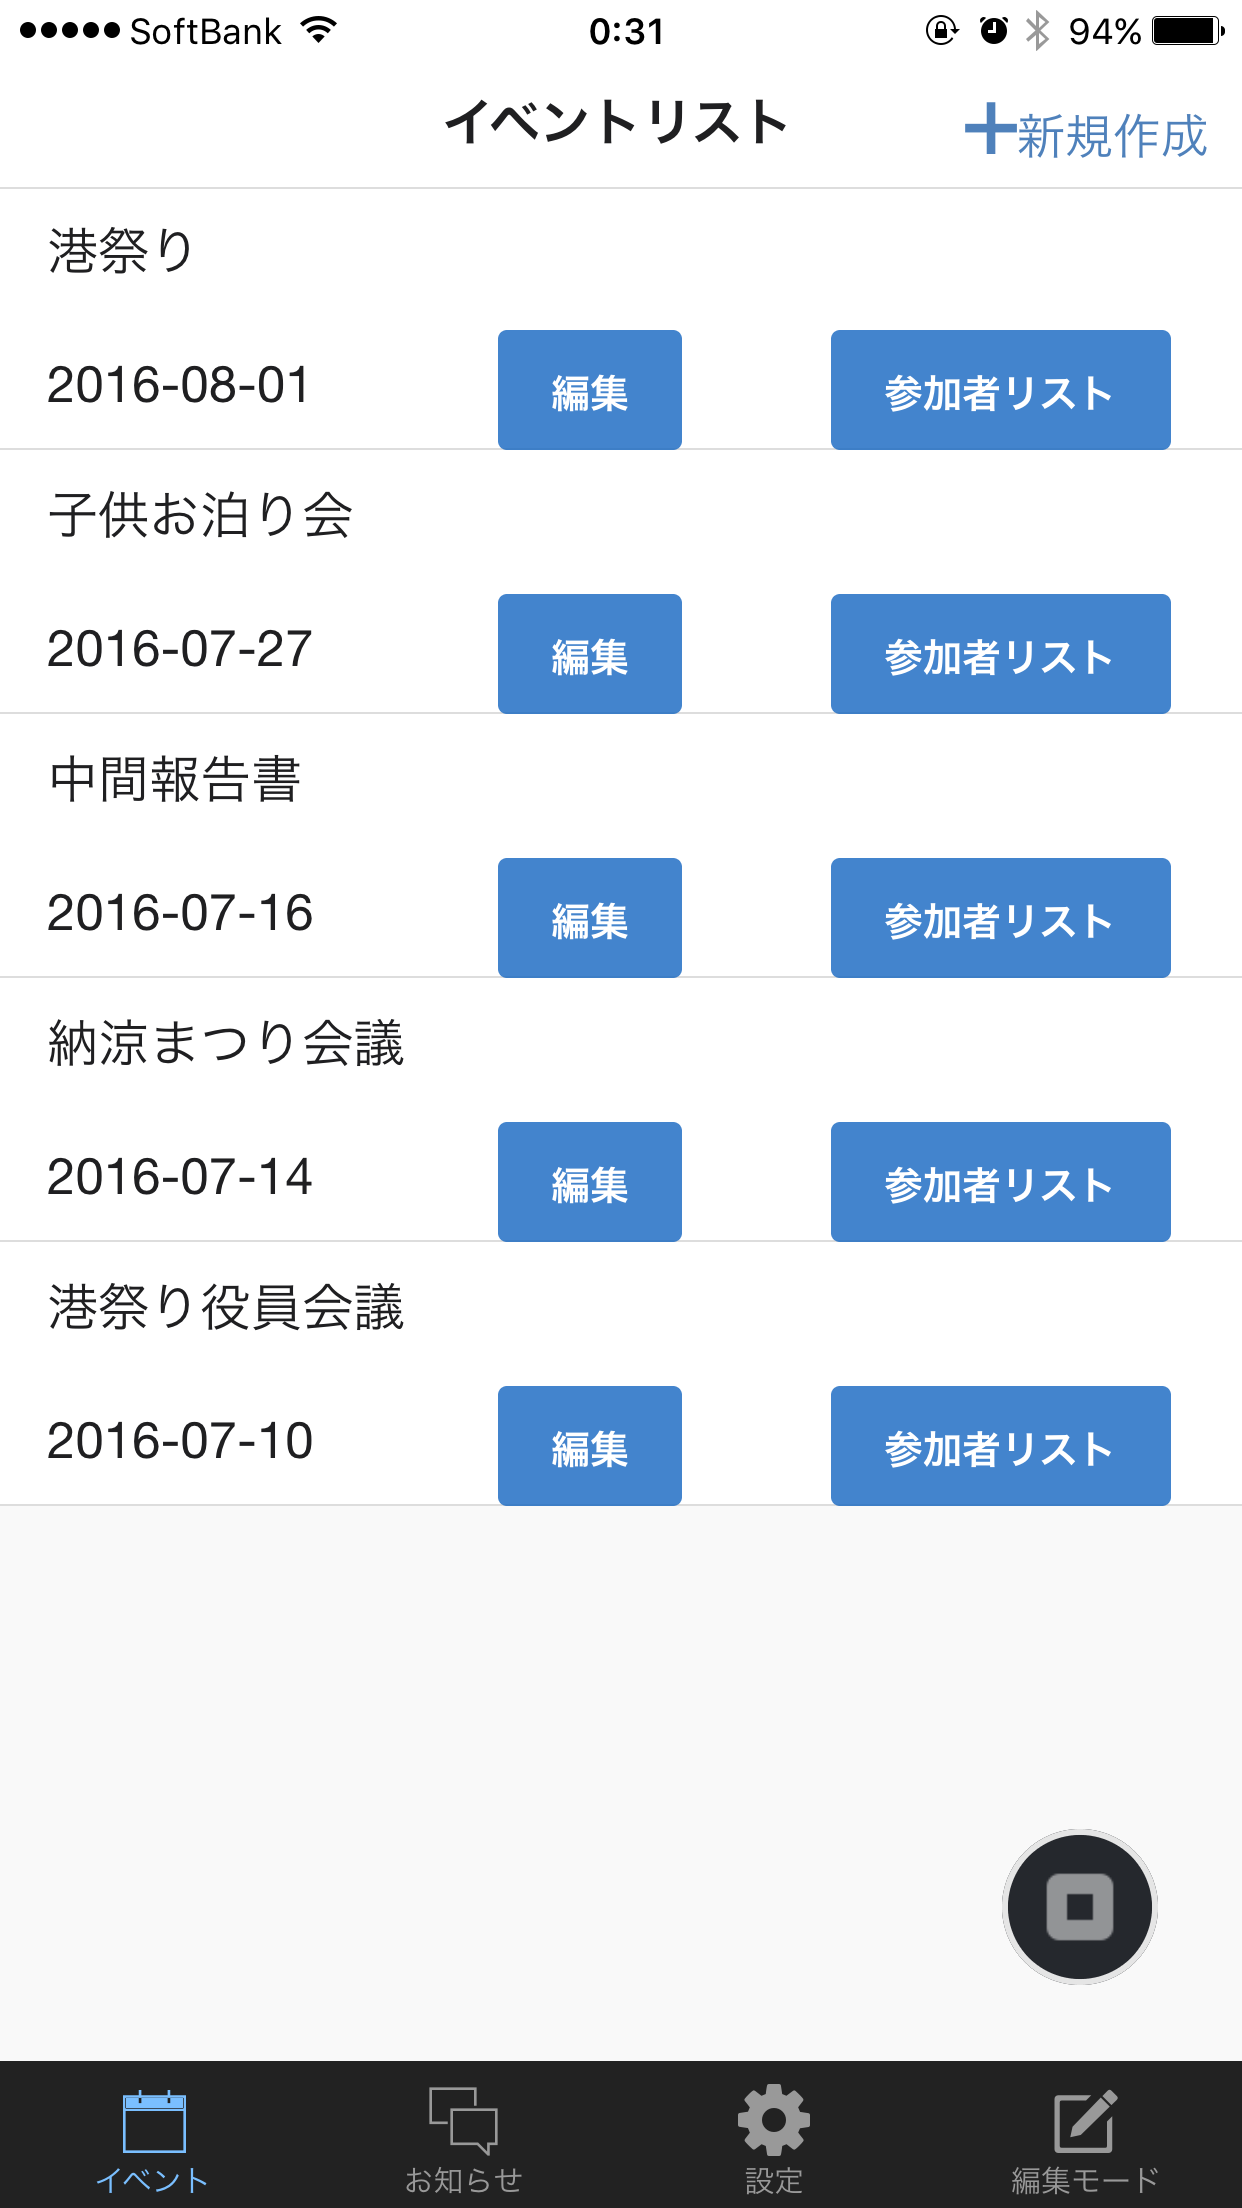
\includegraphics[width=4cm]{event_list.PNG}}}
          \hspace{1cm} %(a)観光スポットの紹介
          {\footnotesize (a)イベント一覧リスト画面}
        \end{center}
      \end{minipage}

      % 2
      \begin{minipage}{0.33\hsize}
        \begin{center}
        {\setlength{\fboxsep}{0cm}\fbox{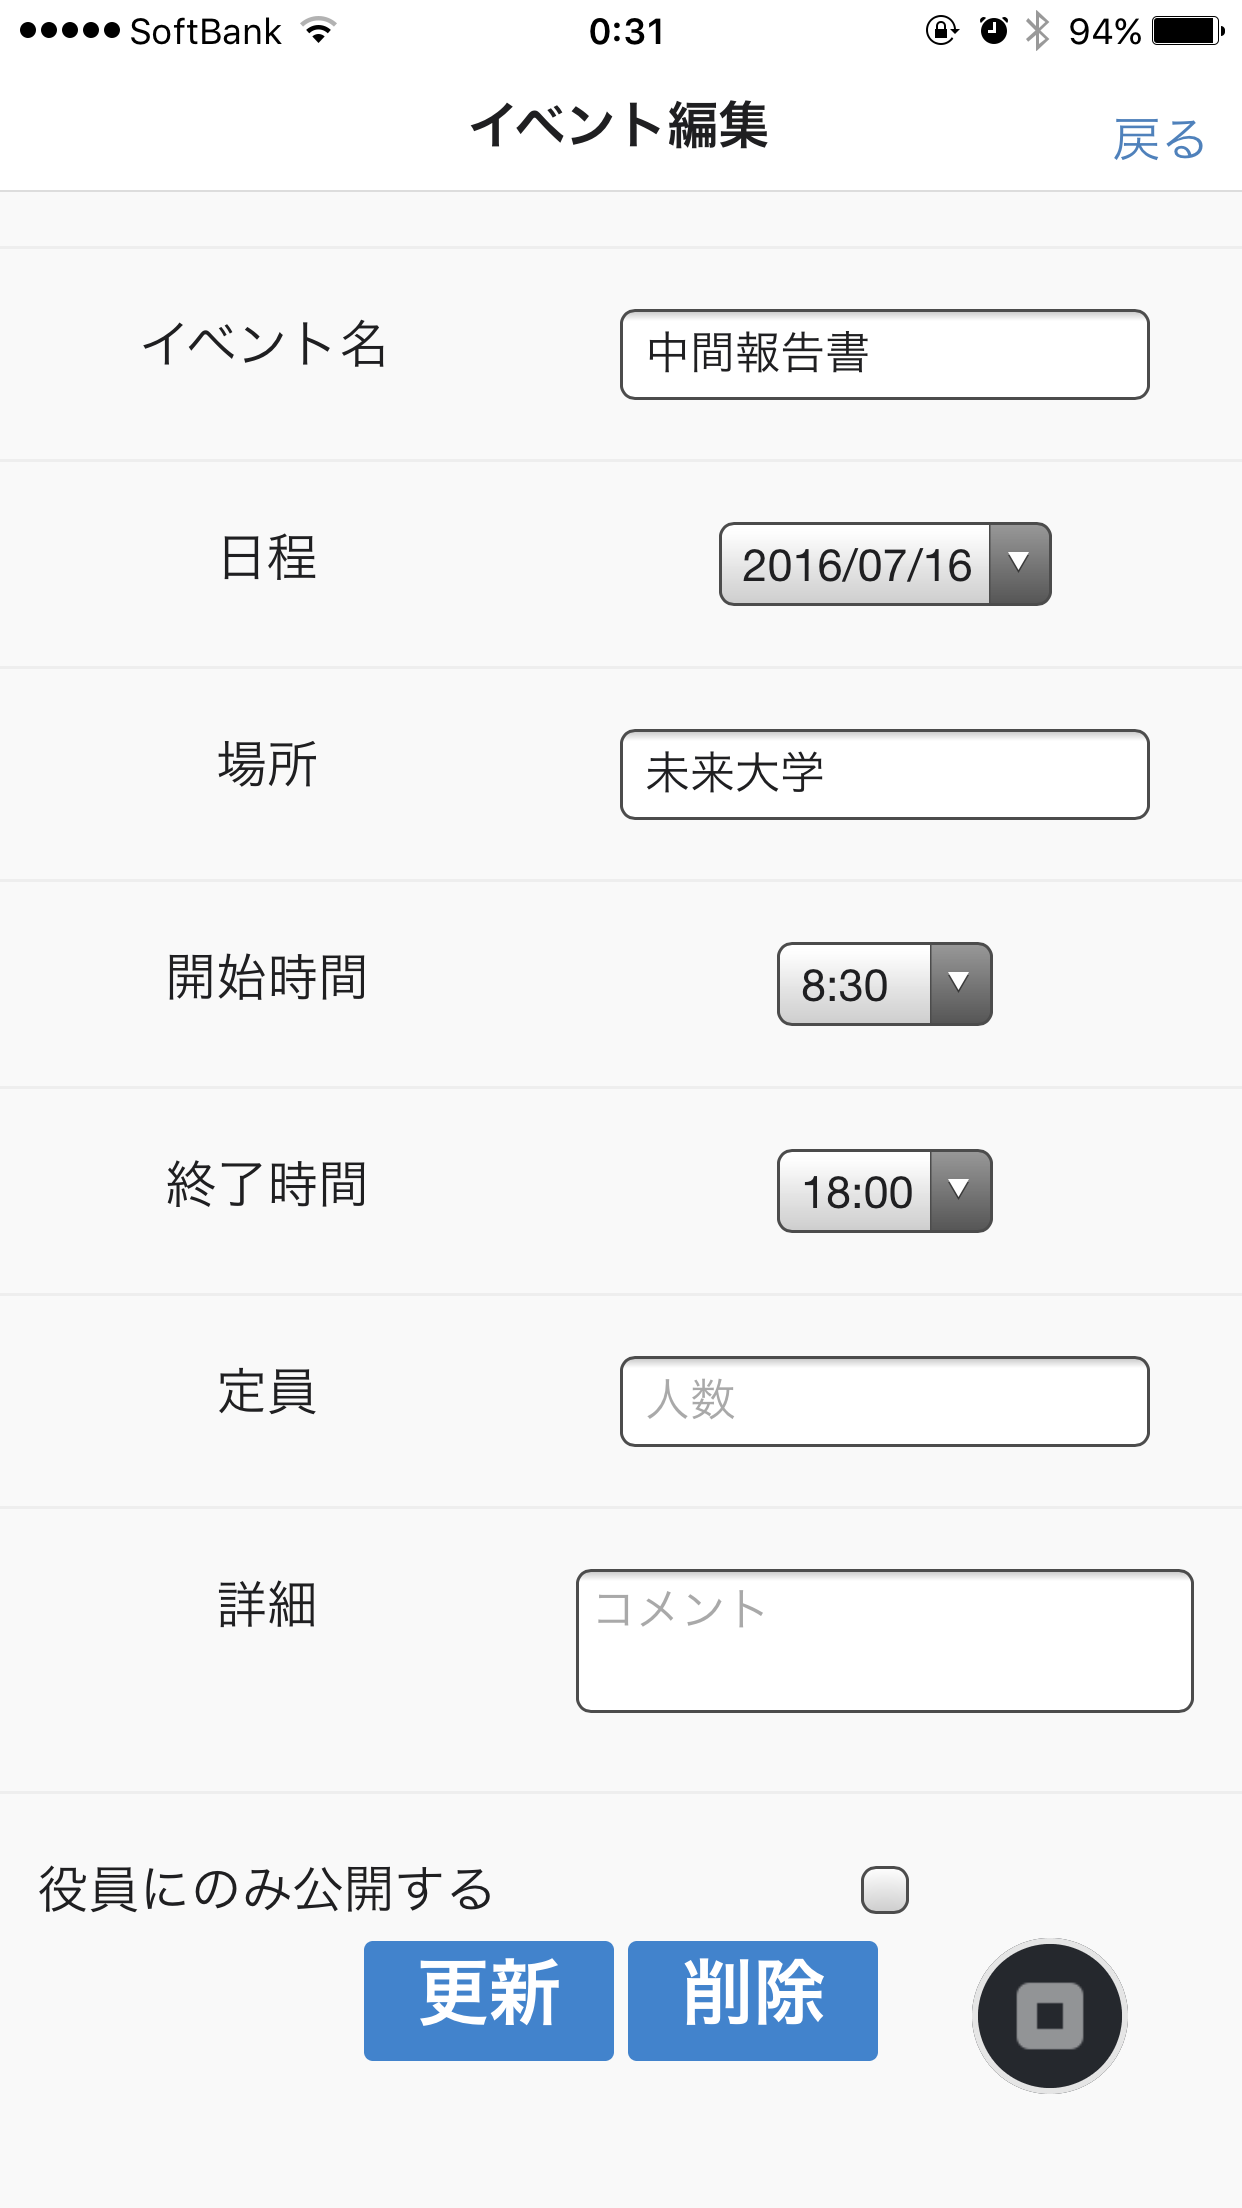
\includegraphics[width=4cm]{event_edit.PNG}}}
          \hspace{1cm}% (b)観光スポットの詳細情報
          {\footnotesize (b)イベント情報の編集画面}
        \end{center}
      \end{minipage}

    \end{tabular}
    \caption{イベント情報の編集}
    \label{tab:edit_event}
  \end{center}
\end{figure}
\bunseki{横山新}

\section{イベント参加申し込み機能}%例:レビュー内容
\subsection{イベント参加申し込み機能の概要}%:発表技法について
イベント参加申し込み機能とはう全てのモードで可能な機能であり, イベントへの参加申し込みを行うことを可能とした. 従来は, 町民がイベントへの参加申し込みをする際に, 電話, メール, FAX等多くの方法が存在していため, 町会は参加者の管理に時間を要していた. イベント参加申し込み機能を実装した理由は, この問題を解決し, 町会の負荷を軽減するためである.

\subsection{イベント参加申し込み画面}%:発表技法について
イベント一覧リスト画面(図\ref{tab:edit_event}(a))から任意のイベントを選択すると, イベント情報の詳細画面(図\ref{tab:edit_event}(b))に遷移する. その後, 画面下の??ボタンを押すと, イベント参加申し込み画面(図\ref{tab:request_event}(b))に遷移する. イベント参加申し込み画面では, 入力する情報の属性として氏名, 性別, 年齢, 電話番号, 住所の5つに分けた. これら5つの属性は, ヒアリングを通して定まったものである. 情報を入力した後画面下の??ボタンを押すことで参加申し込みが可能となる. また, 入力した情報を端末に保存することで, 次回以降の入力を省略することができるようにした。

\begin{figure}[htbp]
  \begin{center}
    \begin{tabular}{c}

      % 1
      \begin{minipage}{0.33\hsize}
        \begin{center}
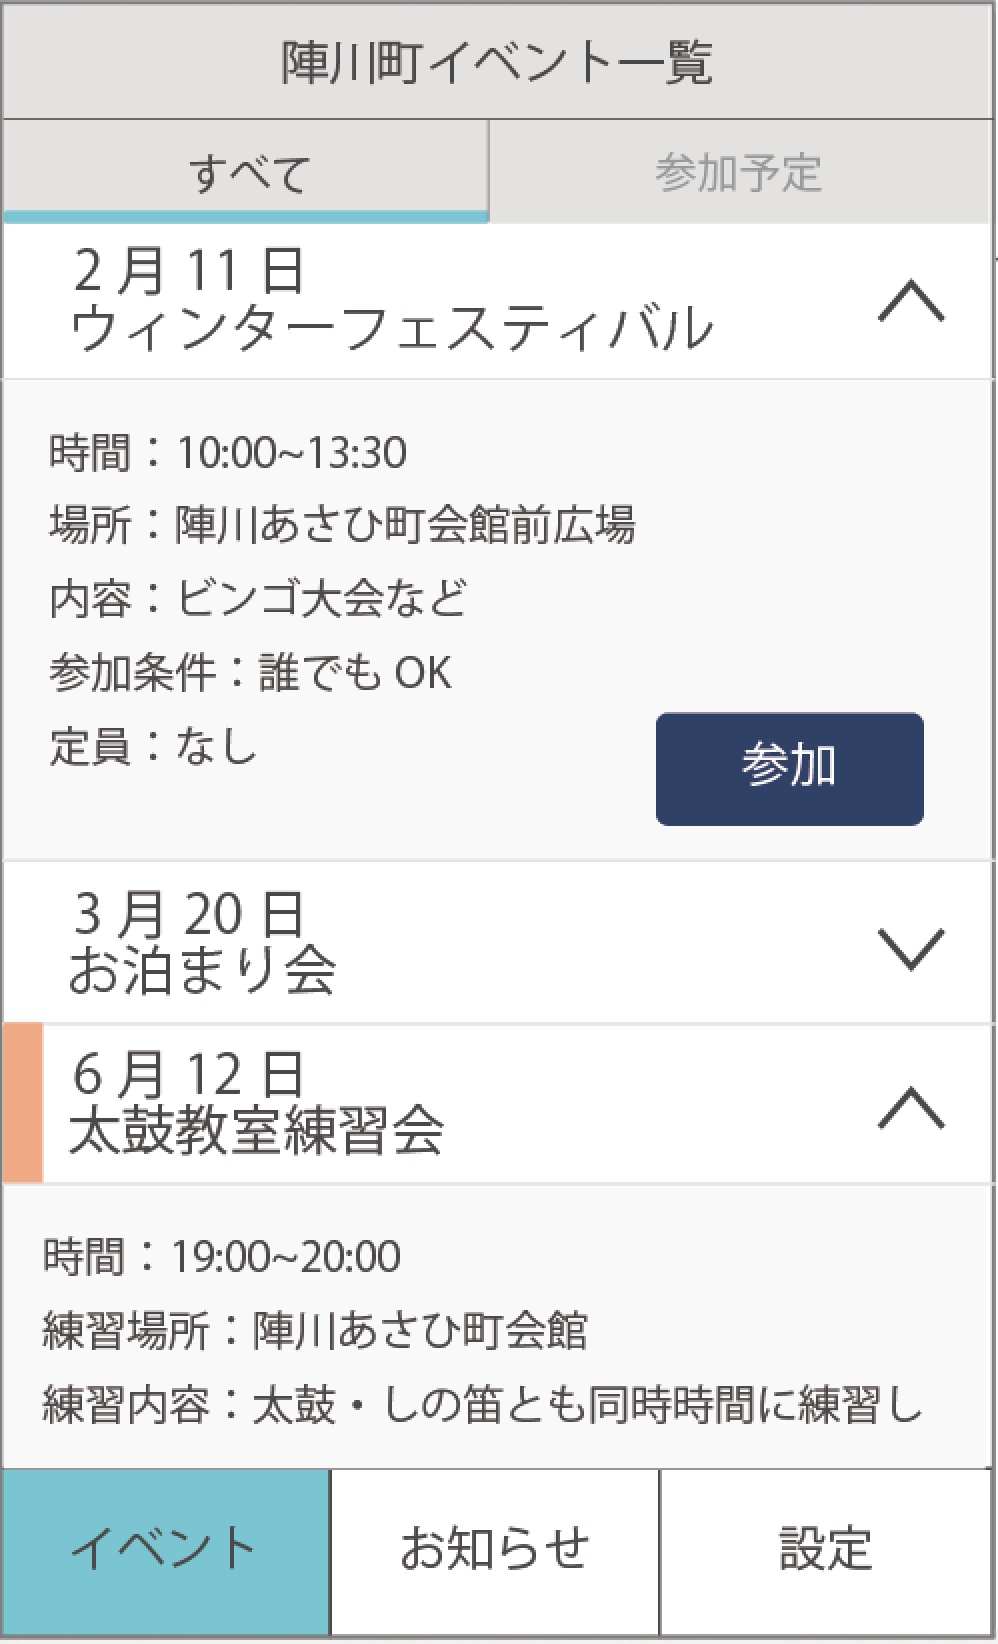
\includegraphics[width=4cm]{event_list_town.png}
          \hspace{1cm} %(a)観光スポットの紹介
          {\footnotesize (a)イベント一覧リスト画面}
        \end{center}
      \end{minipage}

      % 2
      \begin{minipage}{0.33\hsize}
        \begin{center}
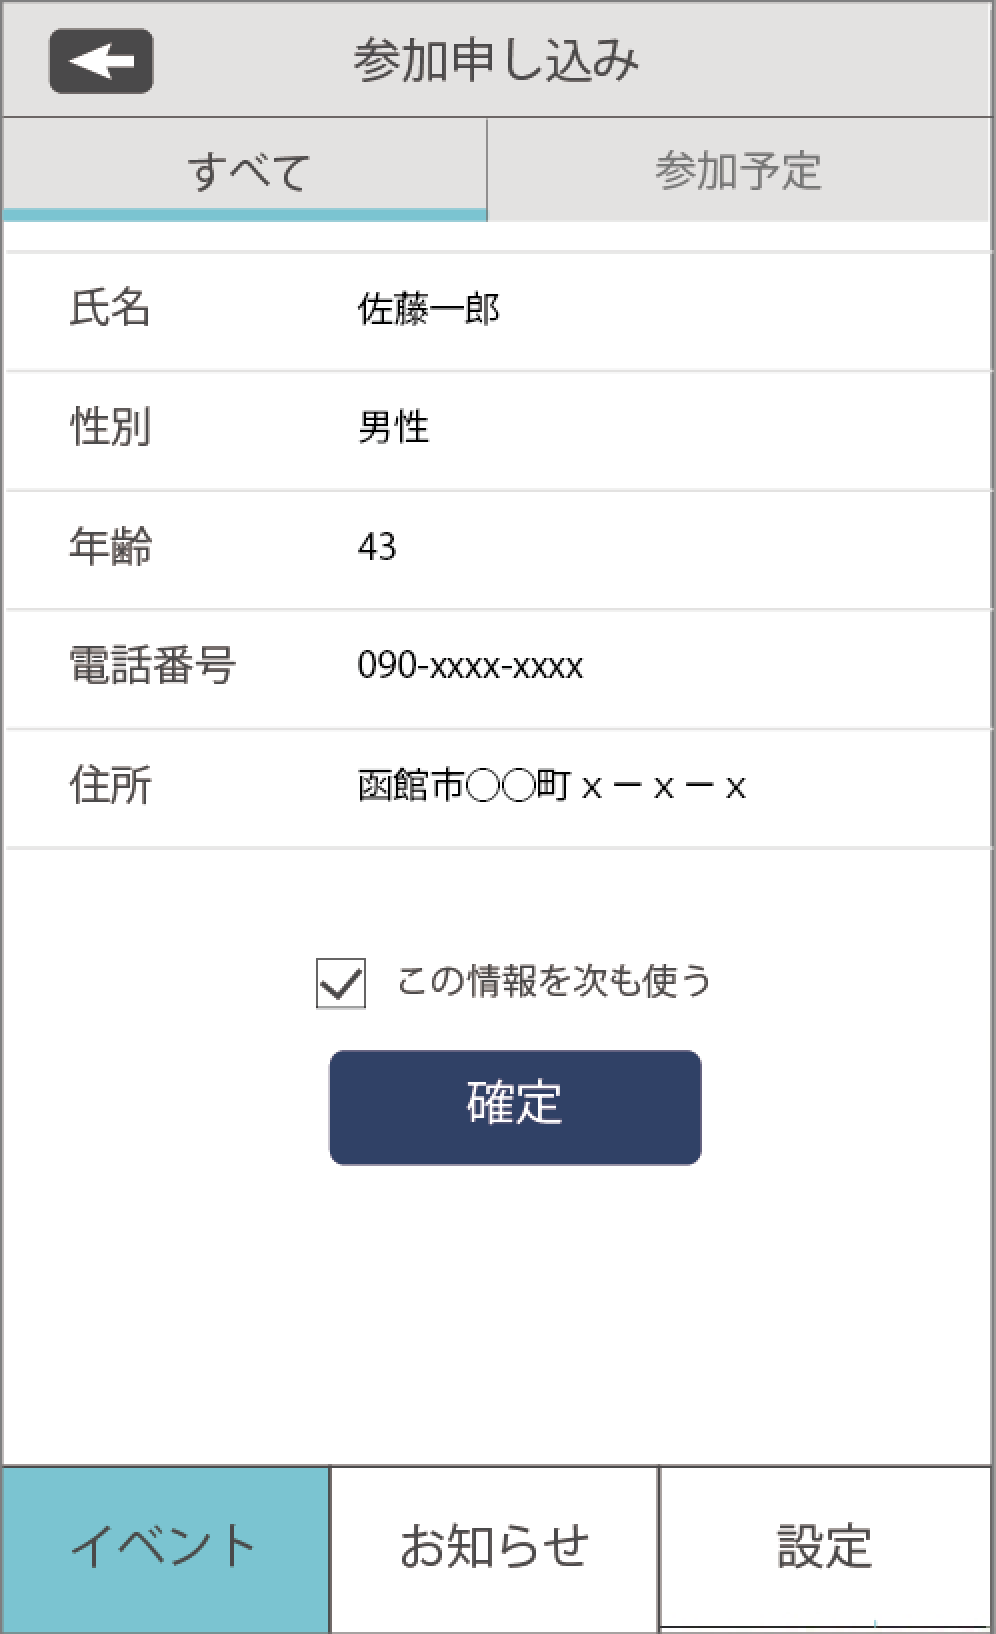
\includegraphics[width=4cm]{participant_form}
          \hspace{1cm}% (b)観光スポットの詳細情報
          {\footnotesize (b)イベント参加申し込み画面}
        \end{center}
      \end{minipage}

    \end{tabular}
    \caption{イベント参加申し込み}
    \label{tab:request_event}
  \end{center}
\end{figure}
\bunseki{横山新}

\section{参加者管理機能}%例:レビュー内容
参加者リスト画面は「役員モード」でのみ閲覧可能な画面(図\ref{tab:joinedlist}(a))であり, イベント毎の参加者一覧の表示や参加取り消しを可能としている. また, 右上のメニューボタンから追加参加ボタンを選択すると, 追加参加画面(図\ref{tab:joinedlist}(b))に遷移する. 実装した理由は, 役員が本アプリケーションを使用することができないユーザの代わりに参加申し込みすることや, イベントの申込み締め切り後に役員がユーザから連絡を受け, 代わりに参加参加申し込みを行えるようにするためである. また, 町会へのヒアリングの結果, 参加者リストを市役所に提出する必要があるイベントが存在することがわかった. これを楽に行えるように, 右上のメニューボタンから??を選択することで, 参加者リストをCSVファイル形式で出力できるようにした. CSVファイルはncmbに保存され, ユーザは画面左上のその他からLINEやGoogleDrive, Dropboxなどに保存することができる.

\begin{figure}[htbp]
  \begin{center}
    \begin{tabular}{c}

      % 1
      \begin{minipage}{0.33\hsize}
        \begin{center}
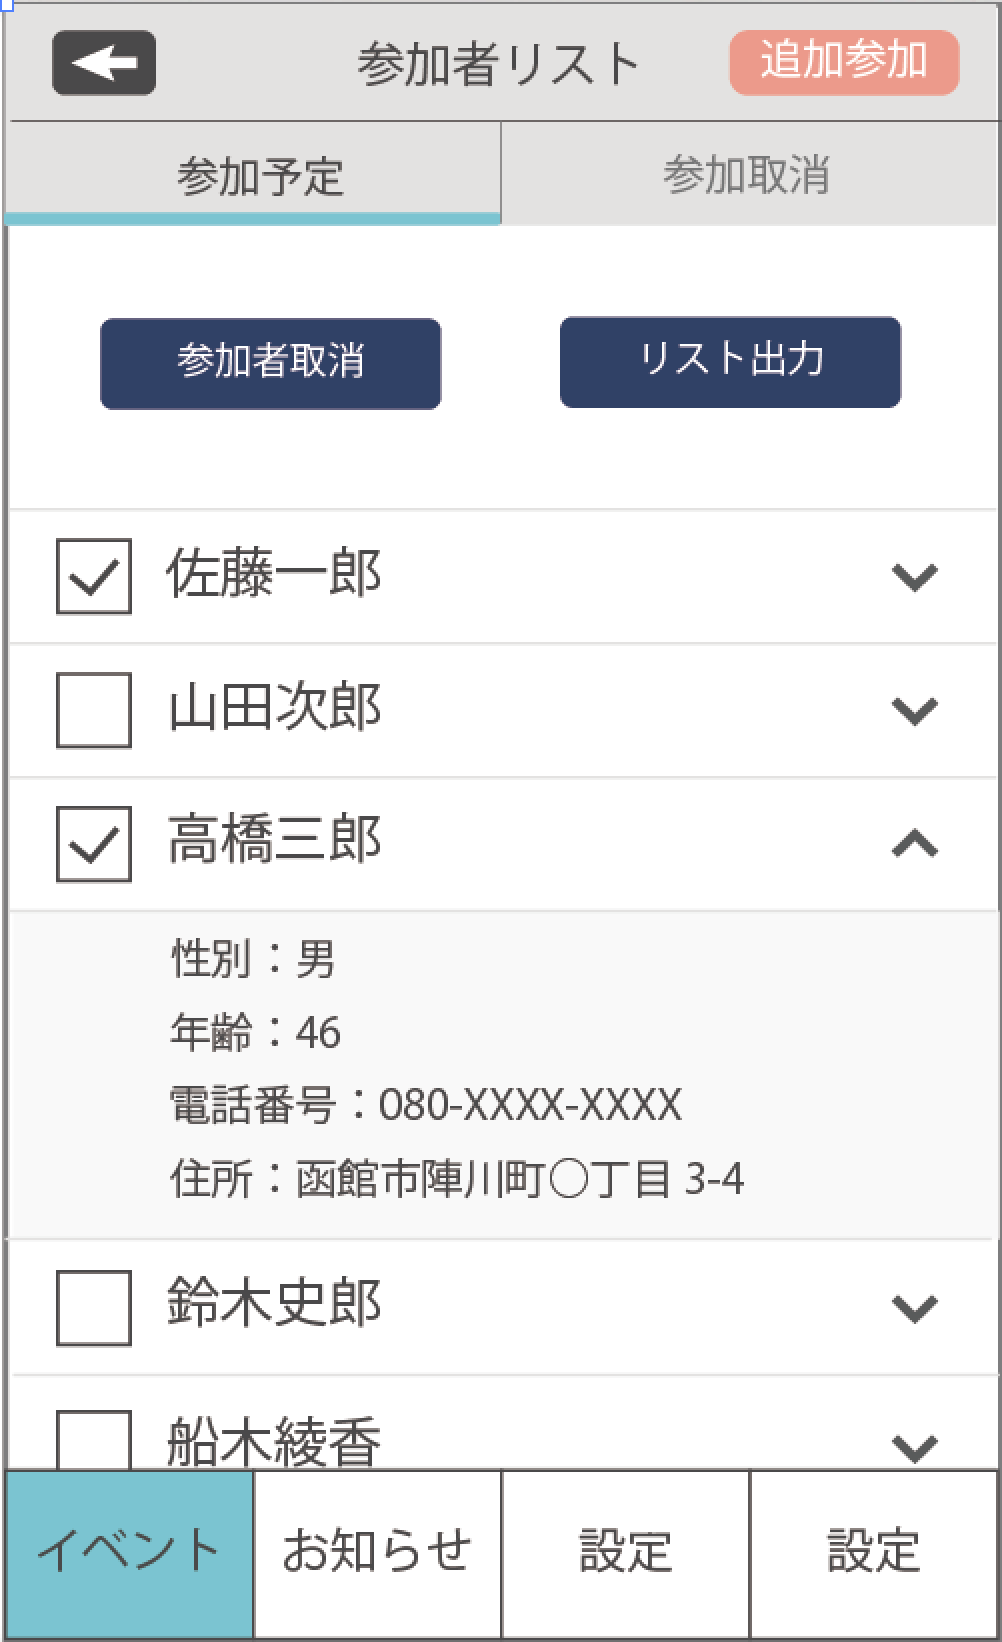
\includegraphics[width=4cm]{participant_list}
          \hspace{1cm} %(a)観光スポットの紹介
          {\footnotesize (a)参加者リスト画面}
        \end{center}
      \end{minipage}

      % 2
      \begin{minipage}{0.33\hsize}
        \begin{center}
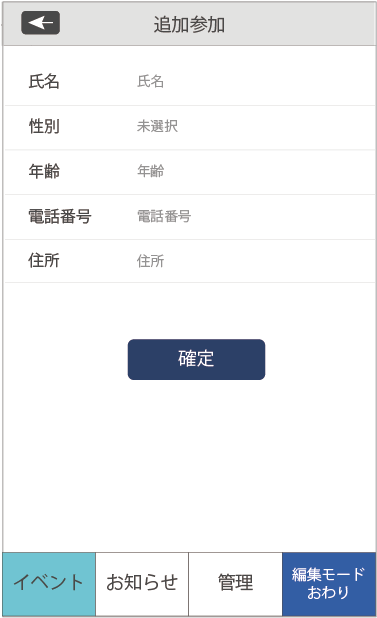
\includegraphics[width=4cm]{participant_add.png}
          \hspace{1cm}% (b)観光スポットの詳細情報
          {\footnotesize (b)追加参加画面}
        \end{center}
      \end{minipage}

    \end{tabular}
    \caption{参加者リスト}
    \label{tab:joinedlist}
  \end{center}
\end{figure}
\bunseki{横山新}

\section{おしらせ管理機能}%例:レビュー内容
\subsection{おしらせ管理機能の概要}%:発表技法について
おしらせ管理機能とは「役員モード」での利用可能な機能であり, 陣川あさひ町会からのお知らせを発信, 発信したお知らせの削除を可能とした. これらは, 管理者のみが使うことを可能とした. おしらせ機能を実装した理由は, \ref{problems}節でも記述したが過去のイベントで雨天中止の連絡ができなかったために, 参加者に風邪を引かせてしまったという事例があったことから, 町会からのお知らせを迅速に参加者に伝える必要があると判断したからである. またこの機能を用いて, 「今日は燃えるゴミが出せる日」「午後から雨が振るので, 洗濯物は取り込んでおいて下さい」といった生活情報の発信も行うことが可能となる.


\subsection{お知らせ作成画面}%:発表技法について
お知らせ一覧リスト画面(図\ref{tab:trans_info}(a))から新規作成ボタンを押すと, お知らせの新規作成画面(図\ref{tab:trans_info}(b))に遷移する. お知らせの新規作成画面では, 担当部名, タイトル, お知らせ内容を入力し役員のみに公開するか否かを選択した後画面下の作成ボタンを押すことでお知らせを発信することが可能となる.

\begin{figure}[htbp]
  \begin{center}
    \begin{tabular}{c}

      % 1
      \begin{minipage}{0.33\hsize}
        \begin{center}
        {\setlength{\fboxsep}{0cm}\fbox{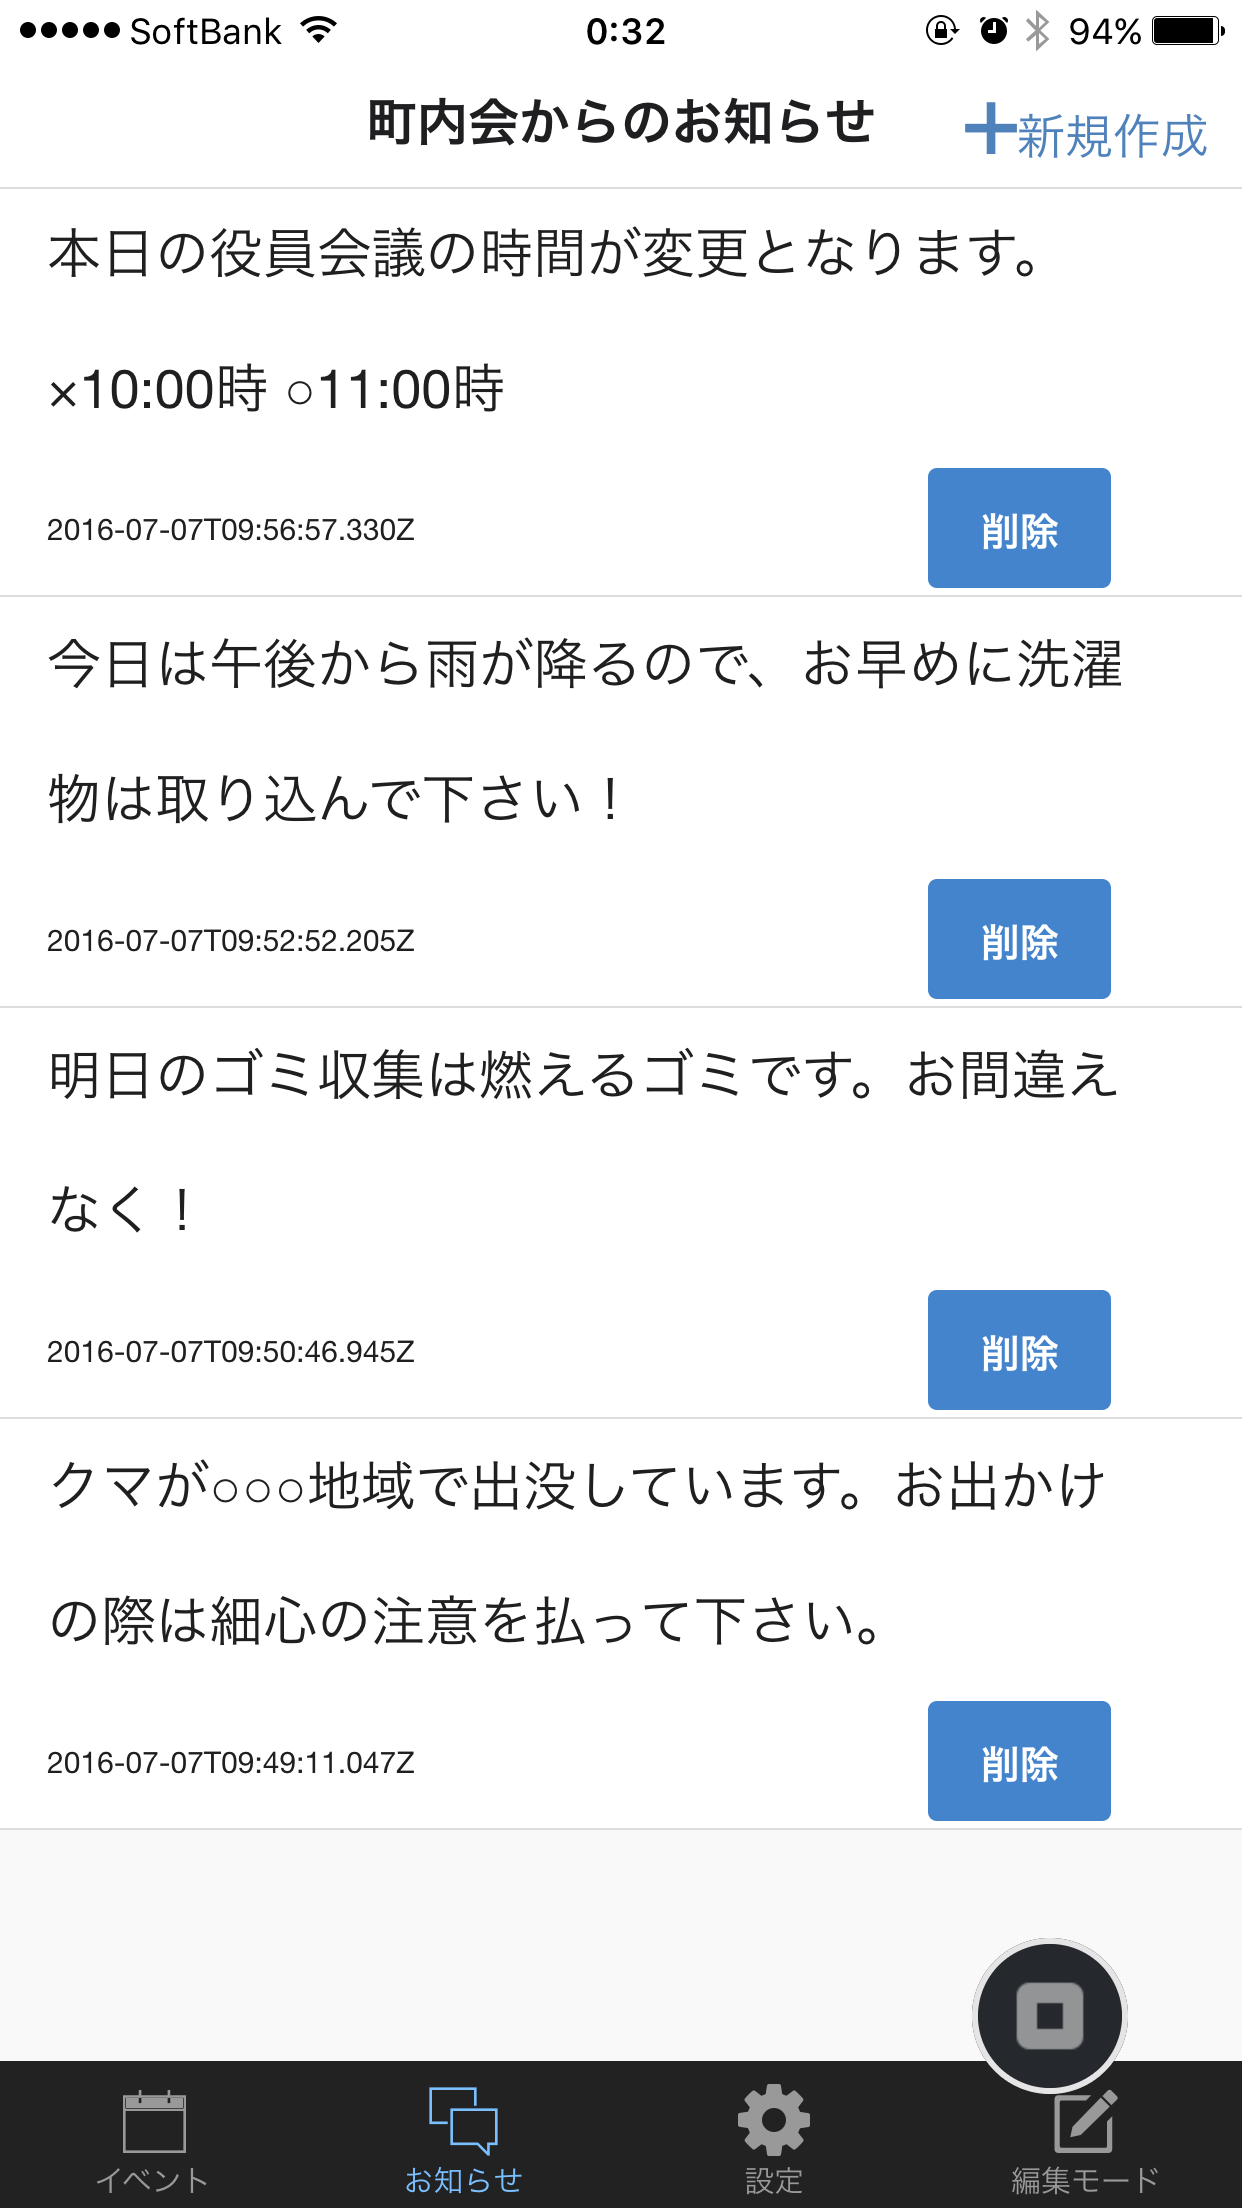
\includegraphics[width=4cm]{notification_list.PNG}
}}
          \hspace{1cm} %(a)観光スポットの紹介
          {\footnotesize (a)お知らせ一覧リスト画面}
        \end{center}
      \end{minipage}

      % 2
      \begin{minipage}{0.33\hsize}
        \begin{center}
         {\setlength{\fboxsep}{0cm}\fbox{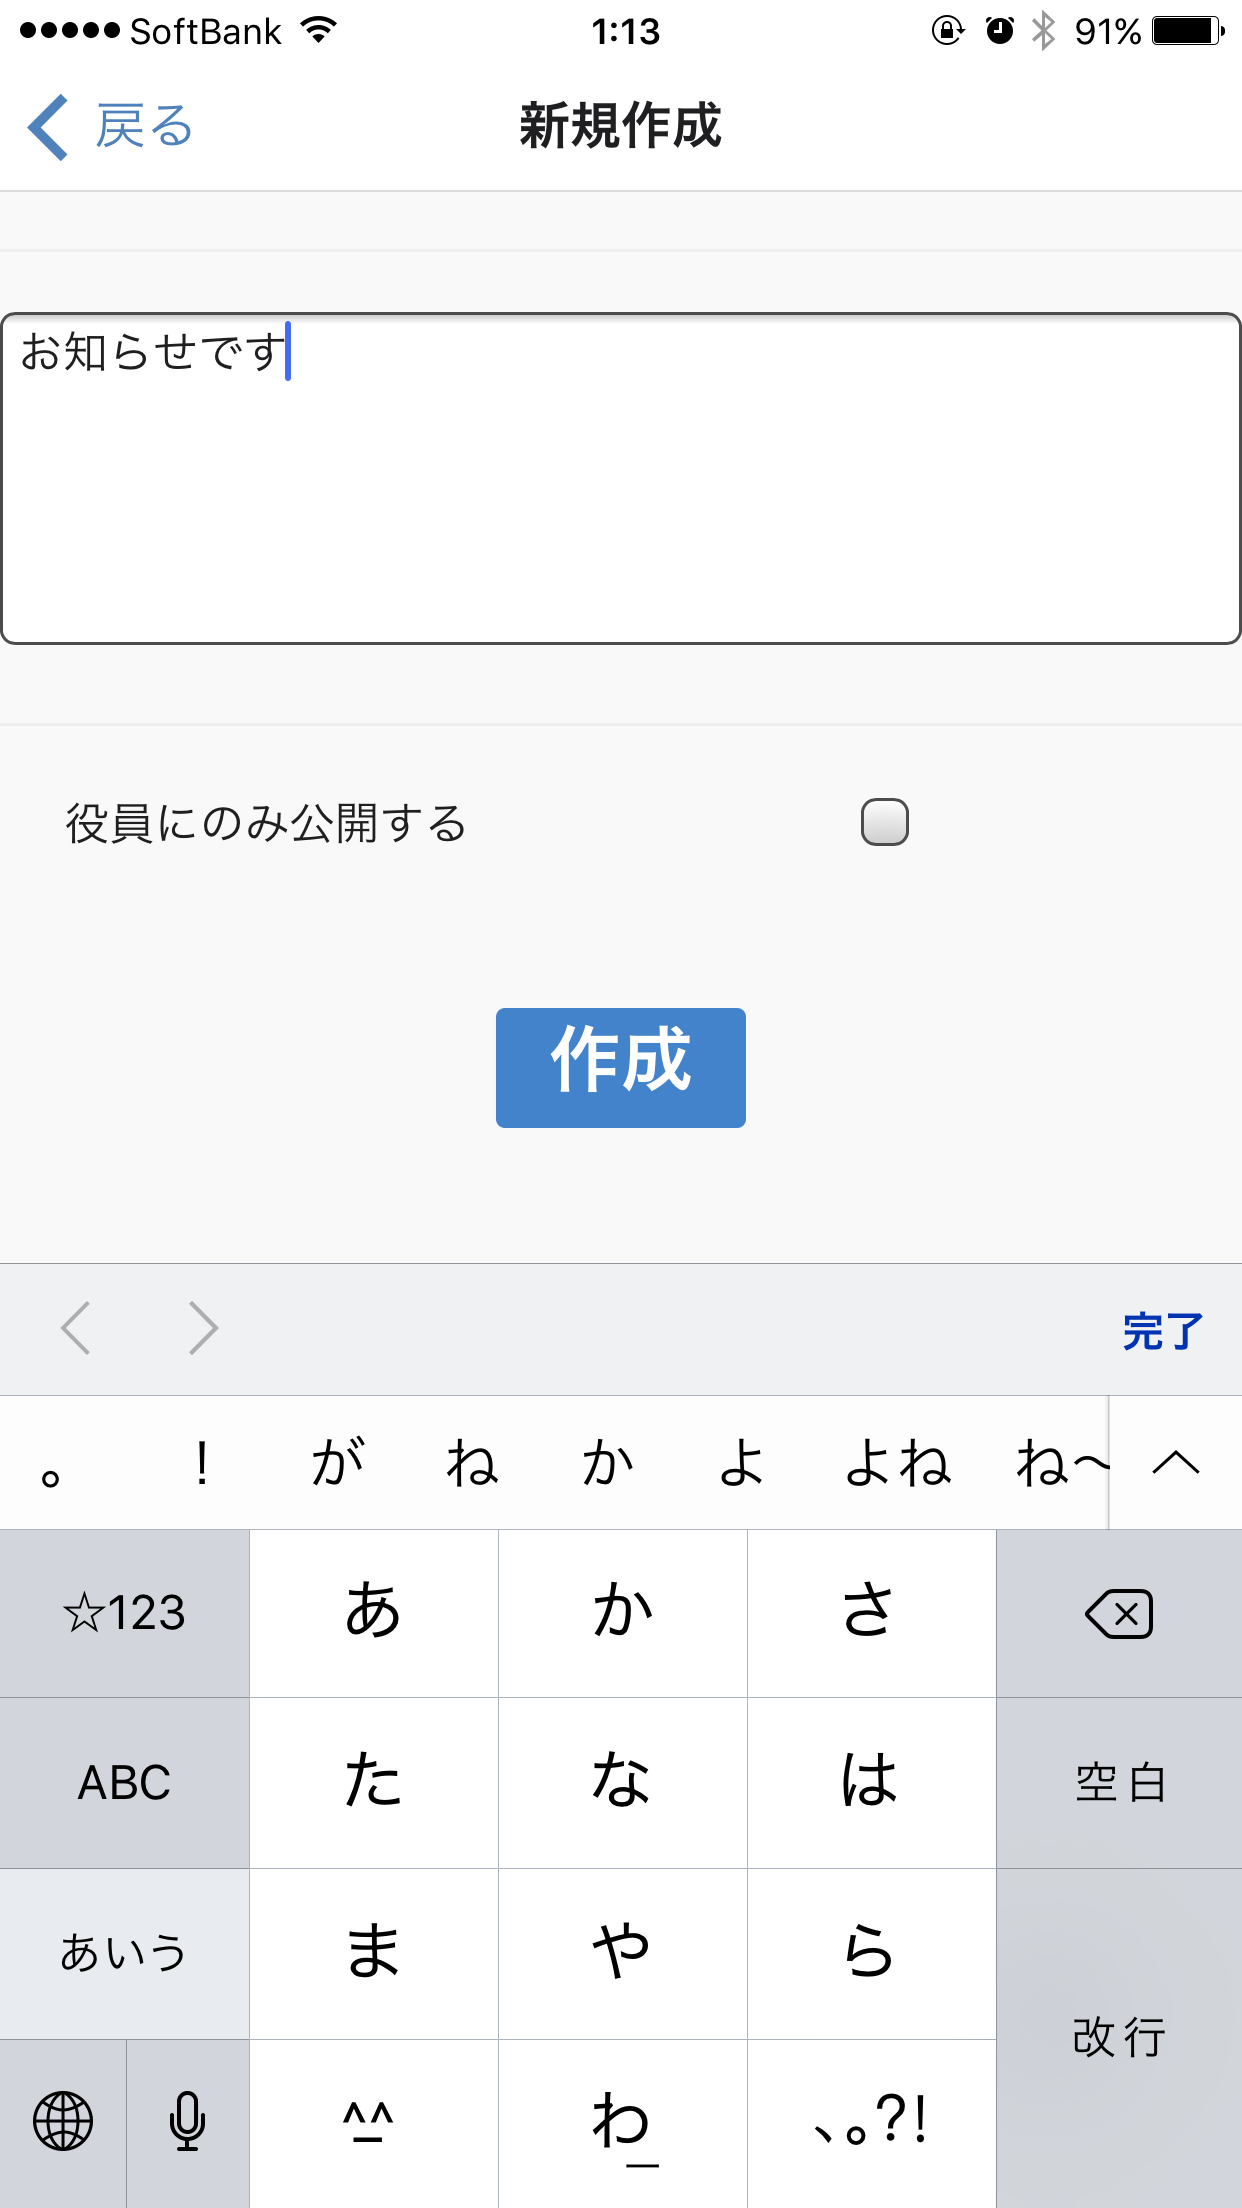
\includegraphics[width=4cm]{notification_add.PNG}}}
          \hspace{1cm}% (b)観光スポットの詳細情報
          {\footnotesize (b)お知らせの新規作成画面}
        \end{center}
      \end{minipage}

    \end{tabular}
    \caption{お知らせ作成}
    \label{tab:trans_info}
  \end{center}
\end{figure}

\subsection{お知らせ削除}%:発表技法について
お知らせ一覧リスト画面(図\ref{fig:delete_info}(a))から削除したいお知らせを選択した後, 削除ボタンを選択して, 発信したお知らせの削除を行う(図\ref{fig:delete_info}(b)).

\begin{figure}[htbp]
  \begin{center}
    \begin{tabular}{c}

      % 1
      \begin{minipage}{0.33\hsize}
        \begin{center}
        {\setlength{\fboxsep}{0cm}\fbox{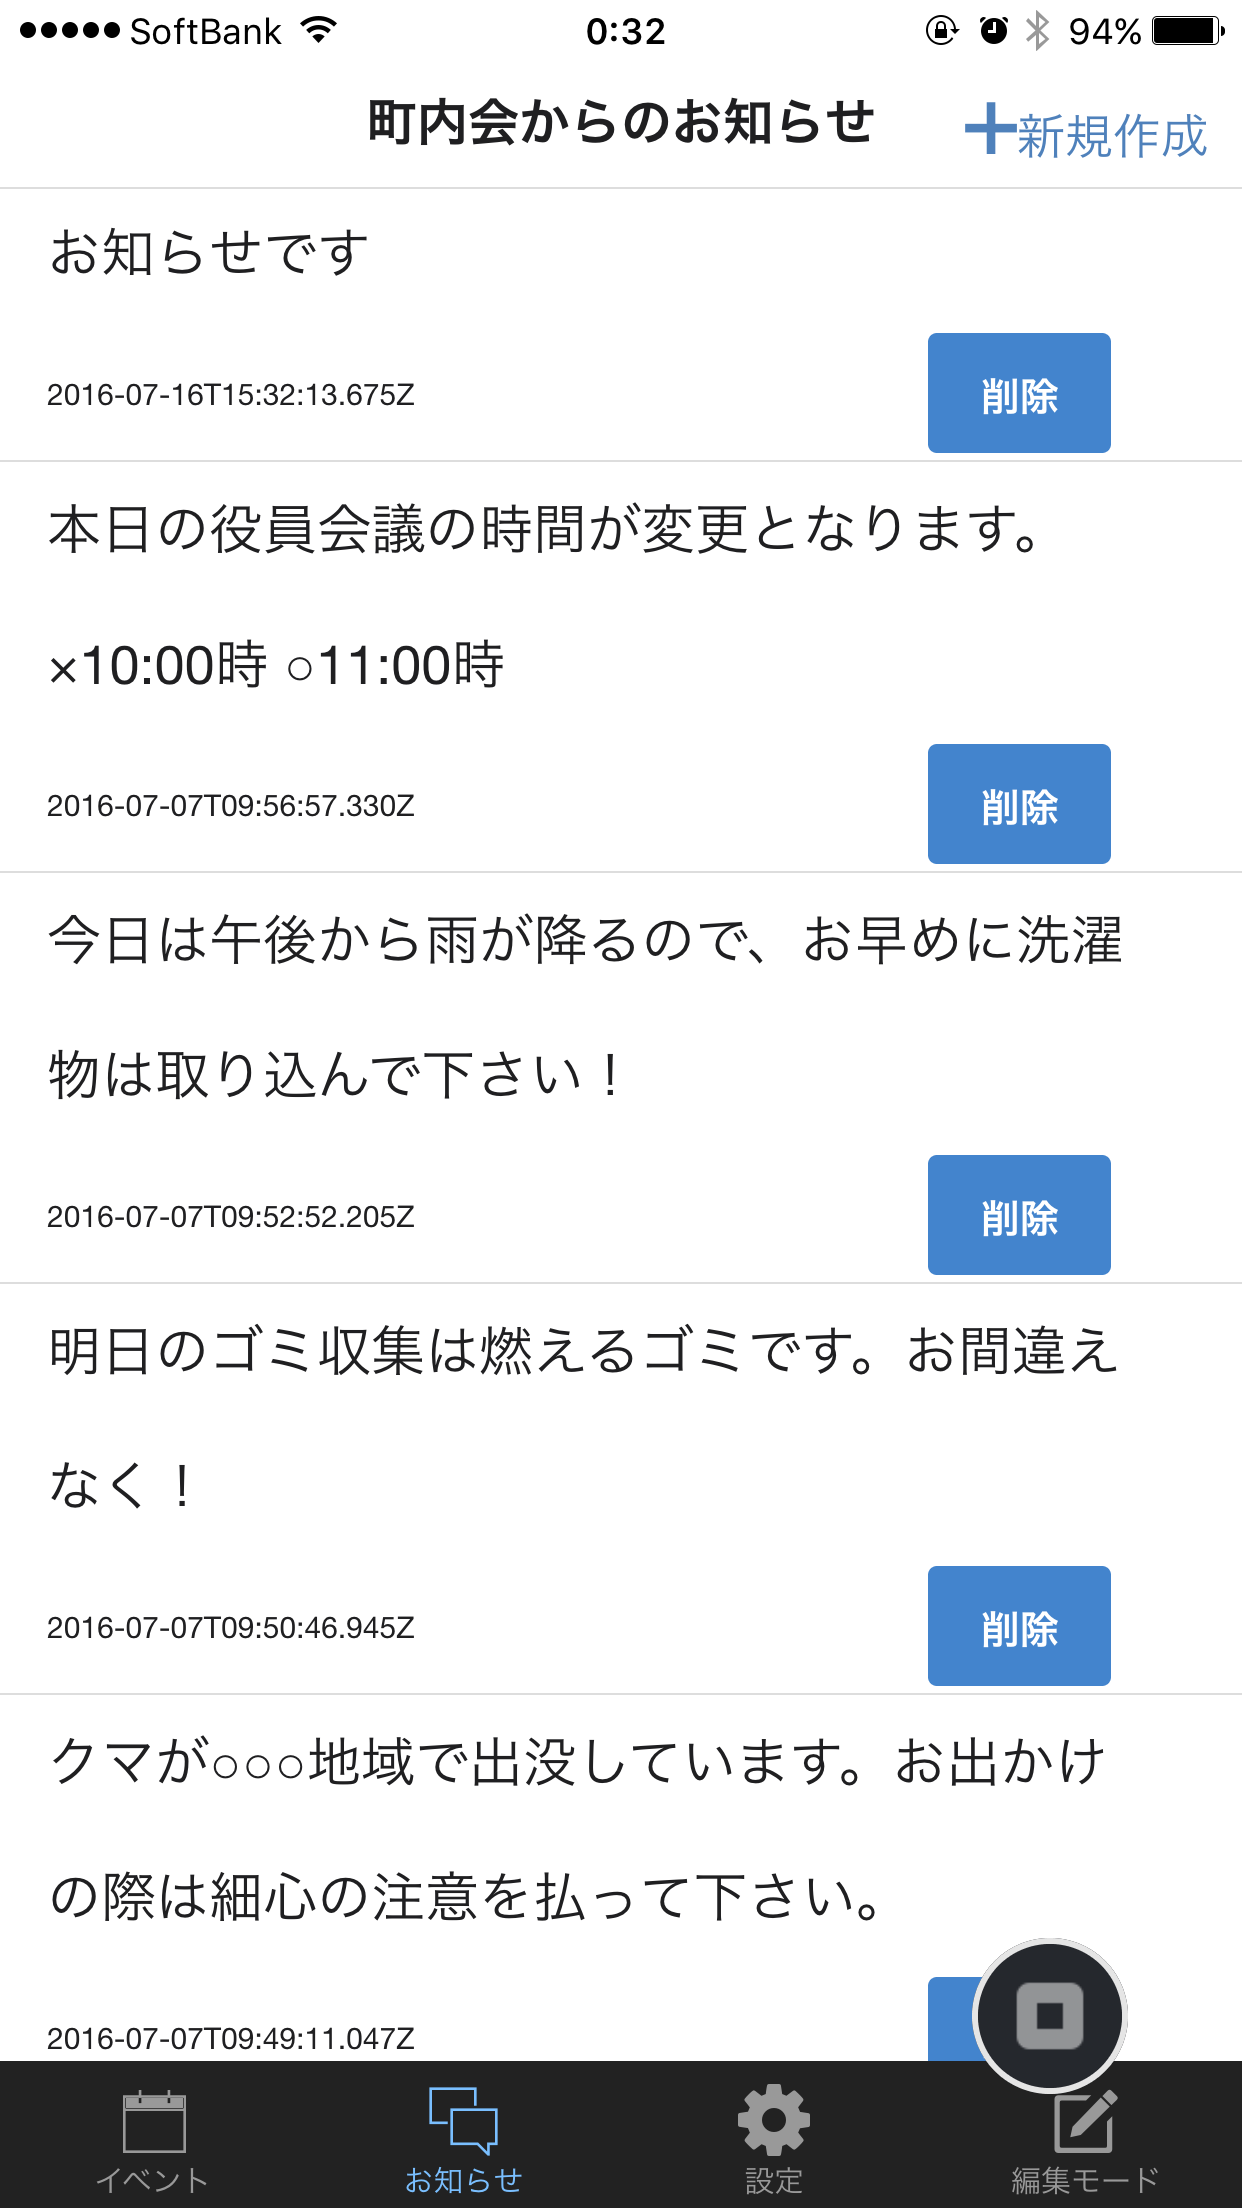
\includegraphics[width=4cm]{notification_list_after_add.PNG}}}
          \hspace{1cm} %(a)観光スポットの紹介
          {\footnotesize (a)お知らせ一覧リスト画面}
        \end{center}
      \end{minipage}

      % 2
      \begin{minipage}{0.33\hsize}
        \begin{center}
        {\setlength{\fboxsep}{0cm}\fbox{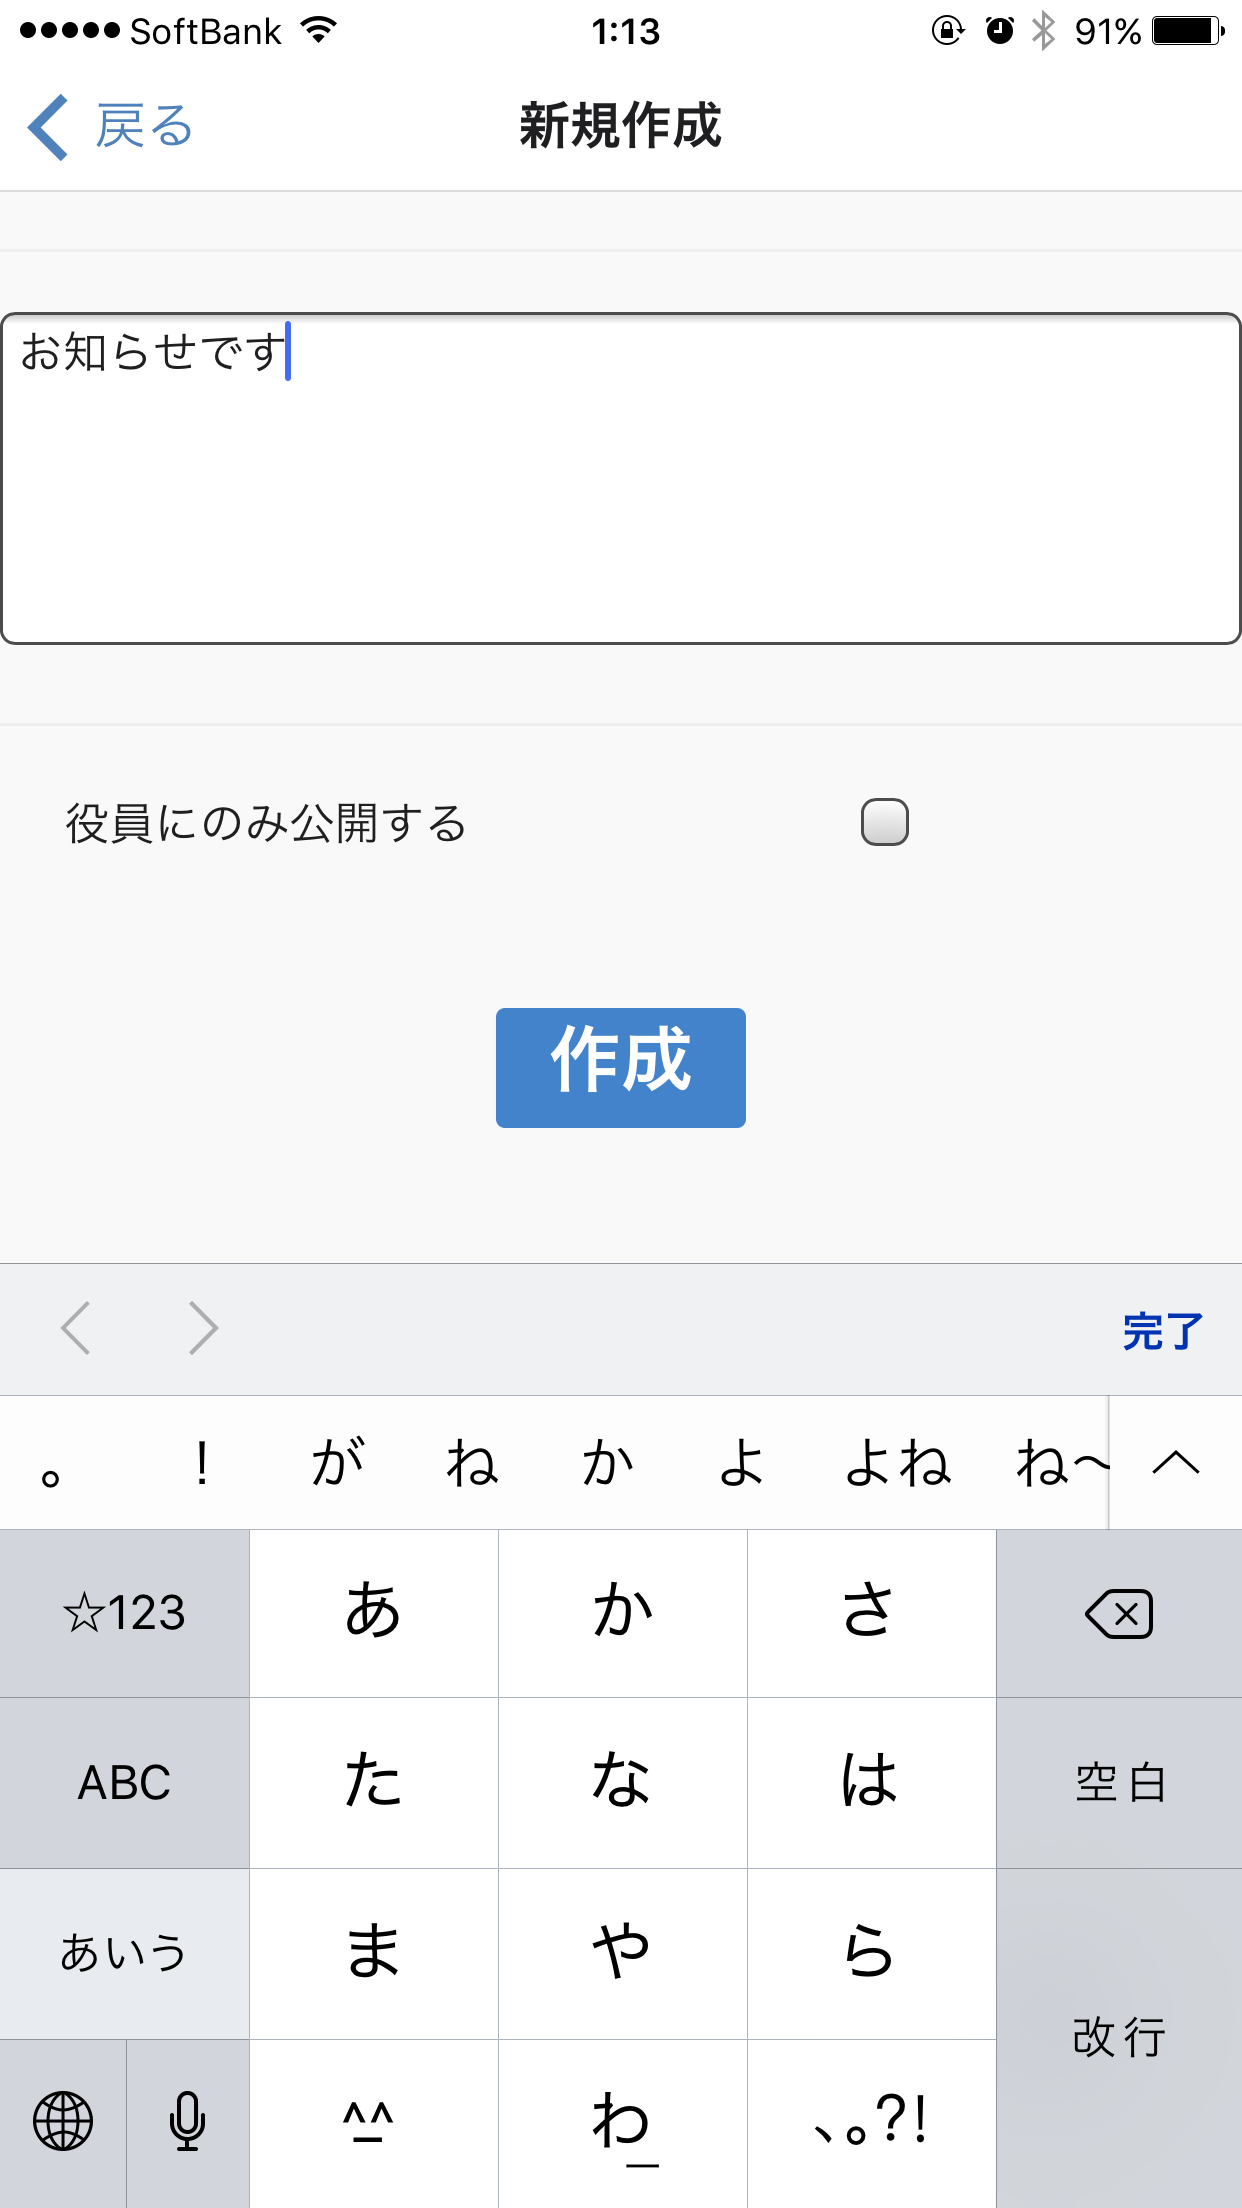
\includegraphics[width=4cm]{notification_add.PNG}}}
          \hspace{1cm}% (b)観光スポットの詳細情報
          {\footnotesize (b)削除を実行した画面}
        \end{center}
      \end{minipage}

    \end{tabular}
    \caption{お知らせ削除}
    \label{fig:delete_info}
  \end{center}
\end{figure}
\bunseki{横山新}


